\documentclass[ignorenonframetext,]{beamer}
\usetheme{Madrid}
\usecolortheme{beaver}
\usepackage{amssymb,amsmath}
\usepackage{ifxetex,ifluatex}
\usepackage{fixltx2e} % provides \textsubscript
\usepackage{lmodern}
\ifxetex
  \usepackage{fontspec,xltxtra,xunicode}
  \defaultfontfeatures{Mapping=tex-text,Scale=MatchLowercase}
  \newcommand{\euro}{€}
\else
  \ifluatex
    \usepackage{fontspec}
    \defaultfontfeatures{Mapping=tex-text,Scale=MatchLowercase}
    \newcommand{\euro}{€}
  \else
    \usepackage[T1]{fontenc}
    \usepackage[utf8]{inputenc}
      \fi
\fi
\IfFileExists{upquote.sty}{\usepackage{upquote}}{}
% use microtype if available
\IfFileExists{microtype.sty}{\usepackage{microtype}}{}
\usepackage{color}
\usepackage{fancyvrb}
\newcommand{\VerbBar}{|}
\newcommand{\VERB}{\Verb[commandchars=\\\{\}]}
\DefineVerbatimEnvironment{Highlighting}{Verbatim}{commandchars=\\\{\}}
% Add ',fontsize=\small' for more characters per line
\usepackage{framed}
\definecolor{shadecolor}{RGB}{248,248,248}
\newenvironment{Shaded}{\begin{snugshade}}{\end{snugshade}}
\newcommand{\KeywordTok}[1]{\textcolor[rgb]{0.13,0.29,0.53}{\textbf{{#1}}}}
\newcommand{\DataTypeTok}[1]{\textcolor[rgb]{0.13,0.29,0.53}{{#1}}}
\newcommand{\DecValTok}[1]{\textcolor[rgb]{0.00,0.00,0.81}{{#1}}}
\newcommand{\BaseNTok}[1]{\textcolor[rgb]{0.00,0.00,0.81}{{#1}}}
\newcommand{\FloatTok}[1]{\textcolor[rgb]{0.00,0.00,0.81}{{#1}}}
\newcommand{\CharTok}[1]{\textcolor[rgb]{0.31,0.60,0.02}{{#1}}}
\newcommand{\StringTok}[1]{\textcolor[rgb]{0.31,0.60,0.02}{{#1}}}
\newcommand{\CommentTok}[1]{\textcolor[rgb]{0.56,0.35,0.01}{\textit{{#1}}}}
\newcommand{\OtherTok}[1]{\textcolor[rgb]{0.56,0.35,0.01}{{#1}}}
\newcommand{\AlertTok}[1]{\textcolor[rgb]{0.94,0.16,0.16}{{#1}}}
\newcommand{\FunctionTok}[1]{\textcolor[rgb]{0.00,0.00,0.00}{{#1}}}
\newcommand{\RegionMarkerTok}[1]{{#1}}
\newcommand{\ErrorTok}[1]{\textbf{{#1}}}
\newcommand{\NormalTok}[1]{{#1}}
\usepackage{url}
\usepackage{letltxmacro}
\makeatletter
\def\maxwidth{\ifdim\Gin@nat@width>\linewidth\linewidth\else\Gin@nat@width\fi}
\def\maxheight{\ifdim\Gin@nat@height>\textheight0.8\textheight\else\Gin@nat@height\fi}
\makeatother
\AtBeginDocument{
  \LetLtxMacro\Oldincludegraphics\includegraphics
  \renewcommand{\includegraphics}[2][]{%
    \Oldincludegraphics[#1,width=\maxwidth,height=\maxheight,keepaspectratio]{#2}}
}

% Comment these out if you don't want a slide with just the
% part/section/subsection/subsubsection title:
\AtBeginPart{
  \let\insertpartnumber\relax
  \let\partname\relax
  \frame{\partpage}
}
\AtBeginSection{
  \let\insertsectionnumber\relax
  \let\sectionname\relax
  \frame{\sectionpage}
}
\AtBeginSubsection{
  \let\insertsubsectionnumber\relax
  \let\subsectionname\relax
  \frame{\subsectionpage}
}

\setlength{\parindent}{0pt}
\setlength{\parskip}{6pt plus 2pt minus 1pt}
\setlength{\emergencystretch}{3em}  % prevent overfull lines
\setcounter{secnumdepth}{0}
\setbeamertemplate{navigation symbols}{}

\title[hwheeler@bsd.uchicago.edu]{Understanding the genetic architecture of gene expression} % The short title appears at the bottom of every slide, the full title is only on the title page

\author{Heather E. Wheeler, PhD} % Your name
\institute[] % Your institution as it will appear on the bottom of every slide, may be shorthand to save space
{
The University of Chicago \\ % Your institution for the title page
\medskip
\textit{hwheeler@bsd.uchicago.edu} % Your email address
}
\date{\today} % Date, can be changed to a custom date

\begin{document}

%\begin{frame}
%\titlepage % Print the title page as the first slide
%\end{frame}

\title{Understanding the genetic architecture of gene expression}
\author{Heather E. Wheeler}
\date{February 13, 2015}

\begin{document}
\frame{\titlepage}

\begin{frame}{PrediXcan Step 1: Build and Test Predictors}

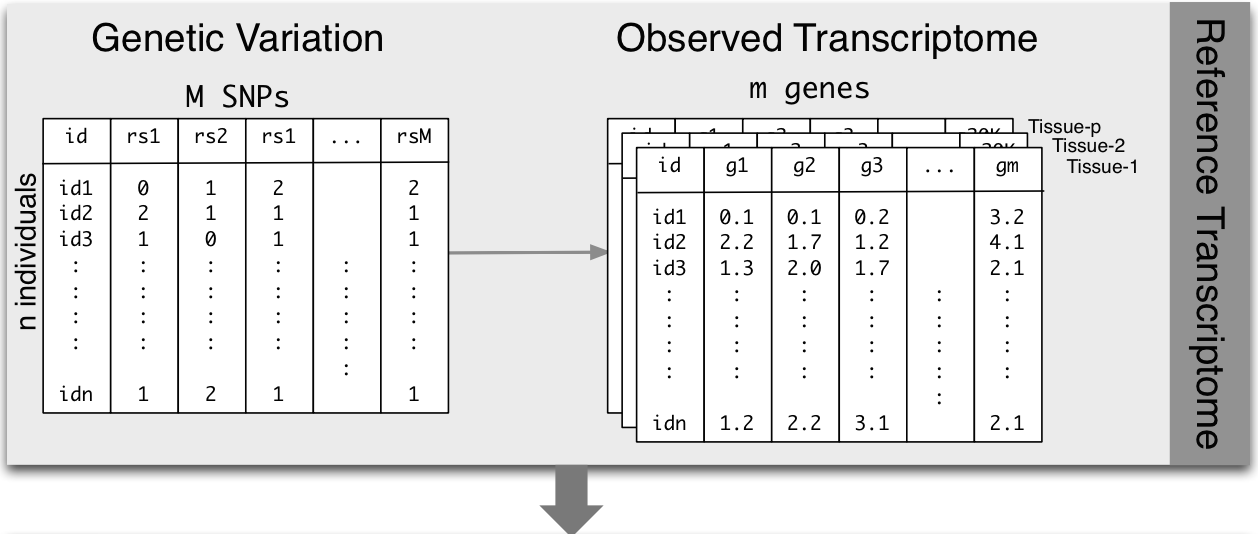
\includegraphics{figs/pred1.png}

\end{frame}

\begin{frame}{PrediXcan Step 2: Build database of Best Predictors}

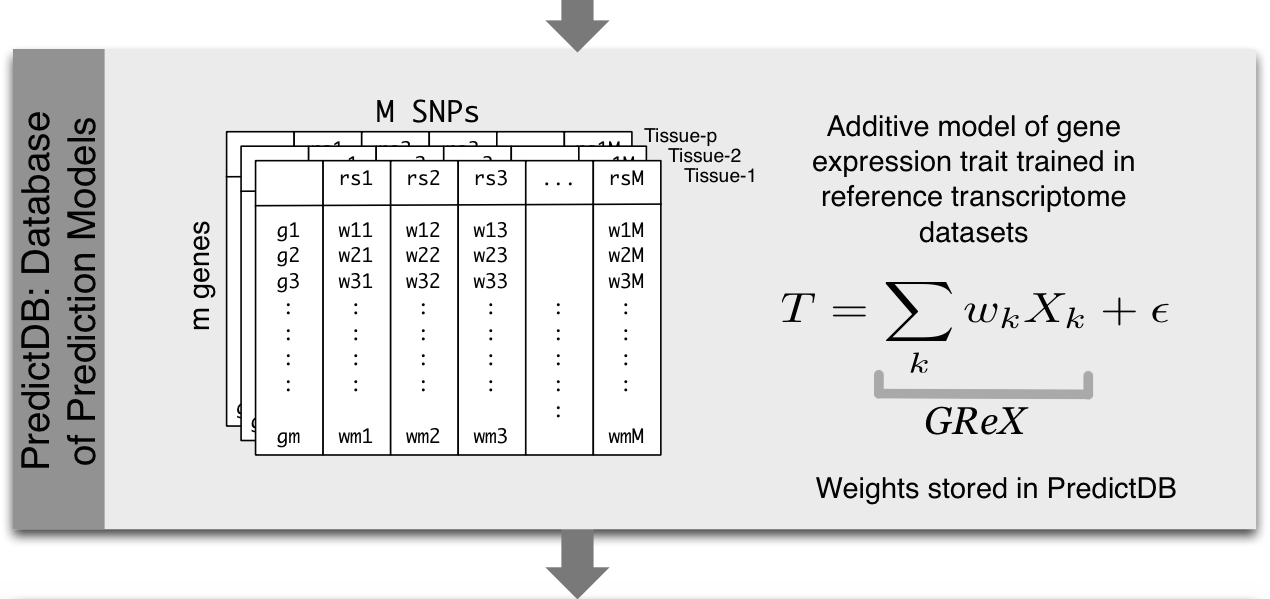
\includegraphics{figs/pred2.png}

\end{frame}

\begin{frame}{PrediXcan Step 3: Impute gene expression and test for
association with phenotype}

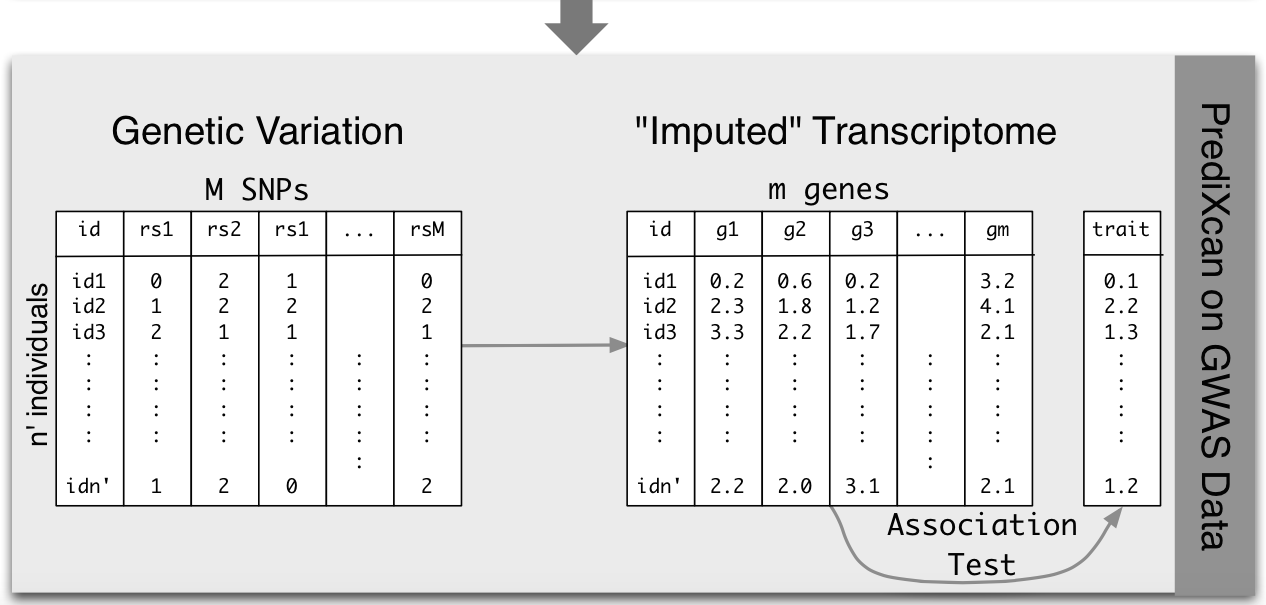
\includegraphics{figs/pred3.png}

\end{frame}

\begin{frame}{Explore the Genetic Architecture of Transcriptome
Regulation}

Optimizing predictors for PrediXcan also tells us about the underlying
genetic architecture of gene expression.

We can ask what proportion of genes have:

\begin{itemize}
\itemsep1pt\parskip0pt\parsep0pt
\item
  \emph{cis} vs. \emph{trans} effects
\item
  sparse vs.~polygenic effects
\item
  cross-tissue vs.~tissue-specific effects
\end{itemize}

\end{frame}

\begin{frame}{Primary cohort: DGN}

\begin{itemize}
\itemsep1pt\parskip0pt\parsep0pt
\item
  Battle et al. ``Characterizing the genetic basis of transcriptome
  diversity through RNA-sequencing of 922 individuals.'' Genome Research
  2014, 24(1):14-24
\item
  Whole blood from Depression Genes and Networks study
\item
  n = 922
\item
  RNA-seq: ``normalized gene-level expression data used for trans-eQTL
  analysis. The data was normalized using HCP (Hidden Covariates with
  Prior) where the parameters were optimized for detecting `trans'
  trends''
\item
  600K genotypes: I have imputed to 1000 Genomes, but some earlier
  analyses were genotyped data only.
\end{itemize}

\end{frame}

\begin{frame}{\emph{cis} vs. \emph{trans} effects}

Estimate the heritability of gene expression in a joint analysis:
localGRM (SNPs w/in 1Mb) + globalGRM (all SNPs)
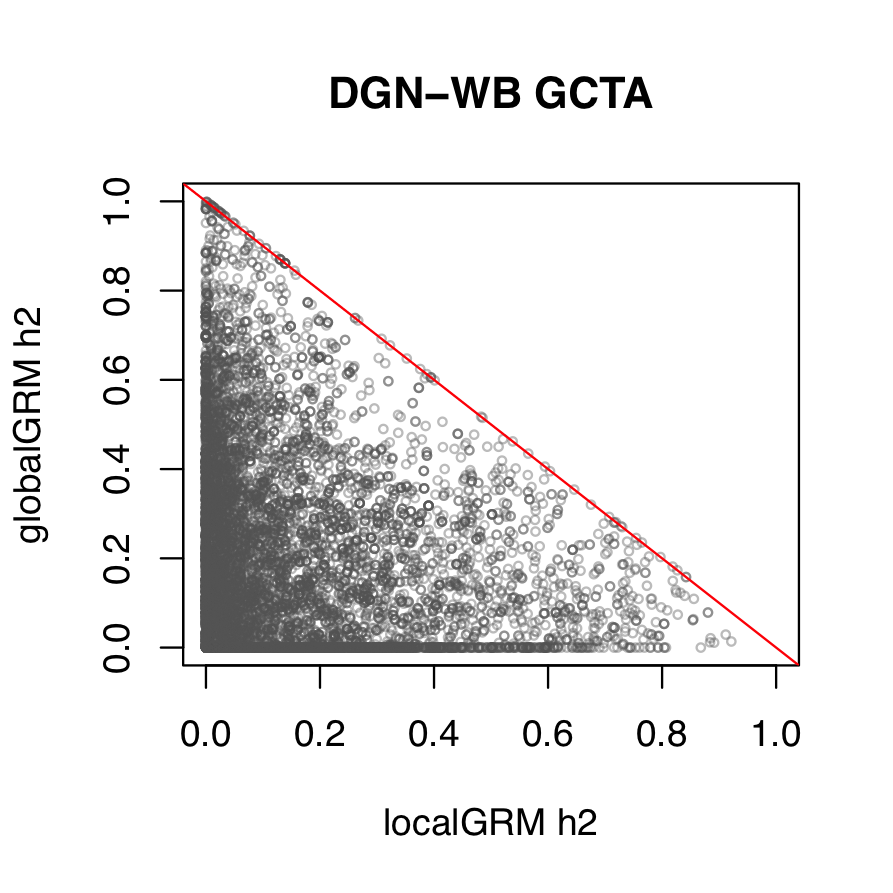
\includegraphics{figs/gcta-DGN-globalvlocal.png}

\end{frame}

\begin{frame}{Local (joint) sorted h\textsuperscript{2} estimates with
95\% CI from GCTA}

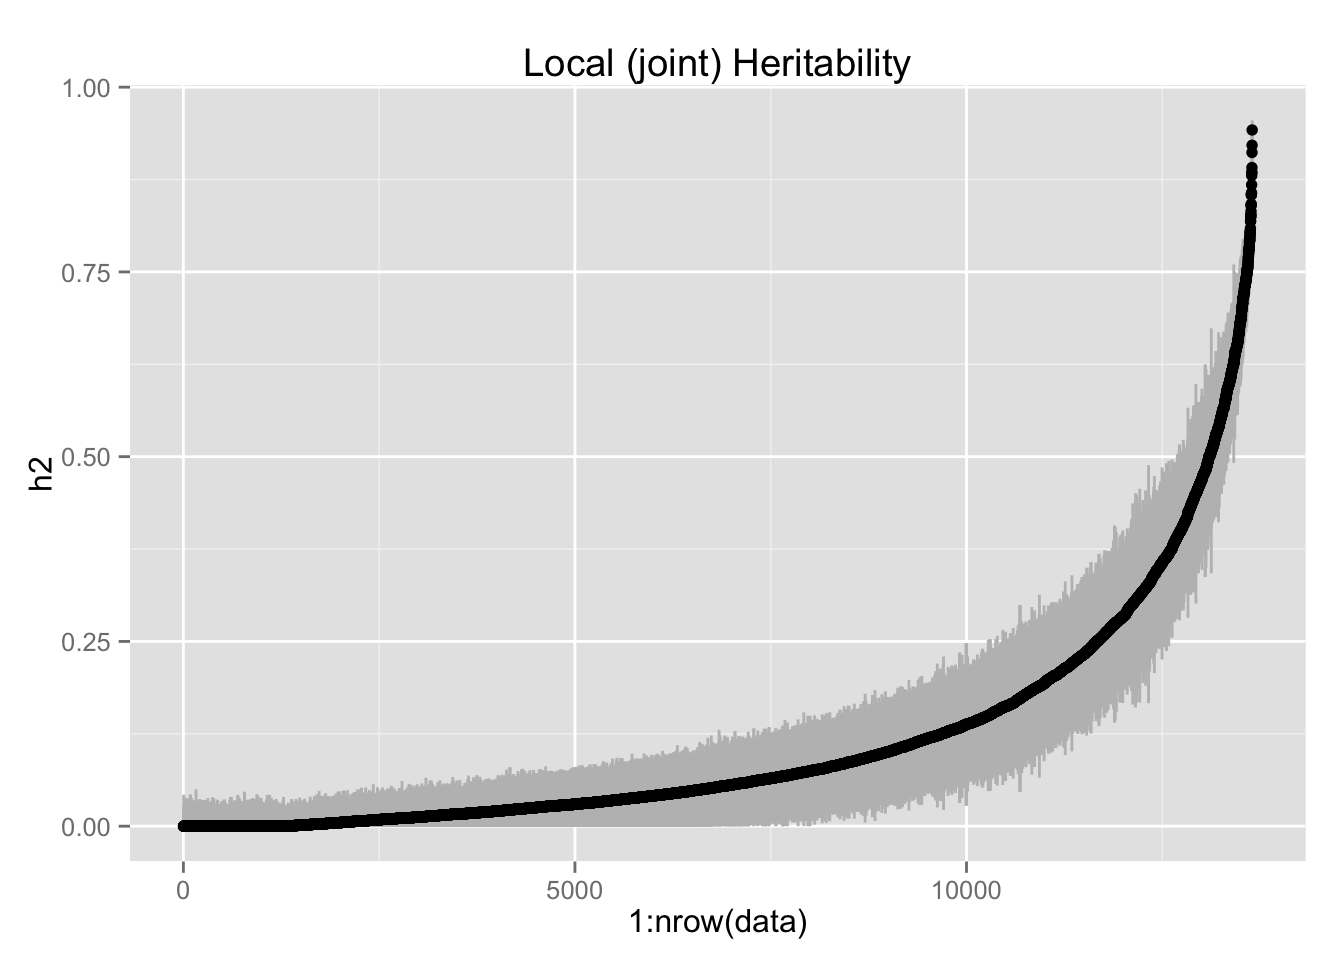
\includegraphics{figs/gcta-DGN-localh2.png}

\tiny \url{https://github.com/hwheeler01/cross-tissue/blob/master/analysis/sources/heritab_analysis.html}

\end{frame}

\begin{frame}{Global (joint) sorted h\textsuperscript{2} estimates with
95\% CI from GCTA}

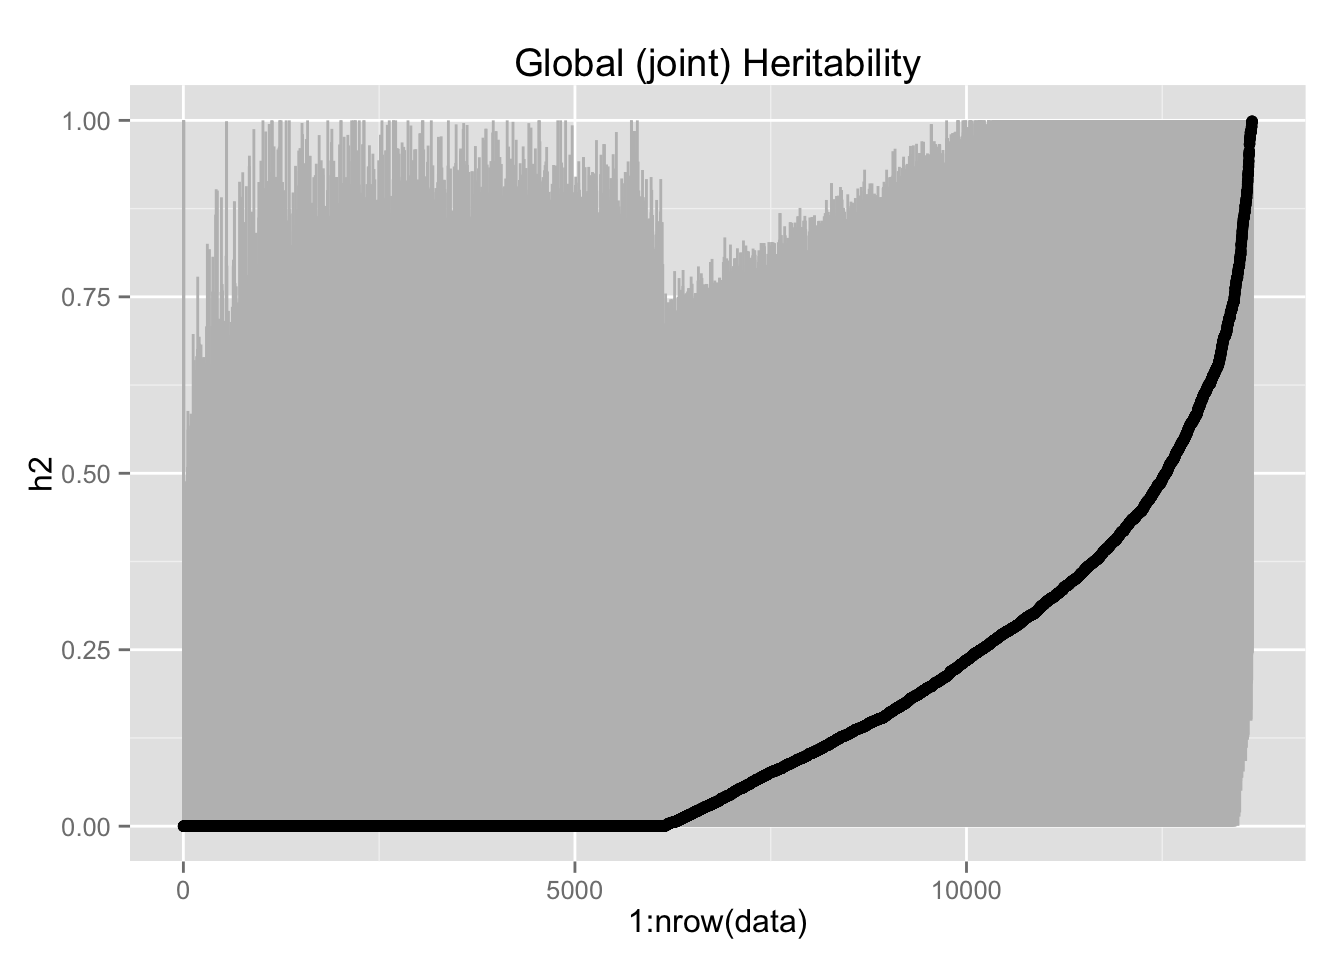
\includegraphics{figs/gcta-DGN-globalh2.png}

\tiny \url{https://github.com/hwheeler01/cross-tissue/blob/master/analysis/sources/heritab_analysis.html}

\end{frame}

\begin{frame}{100 permutations to determine expected distribution of
h\textsuperscript{2} estimates}

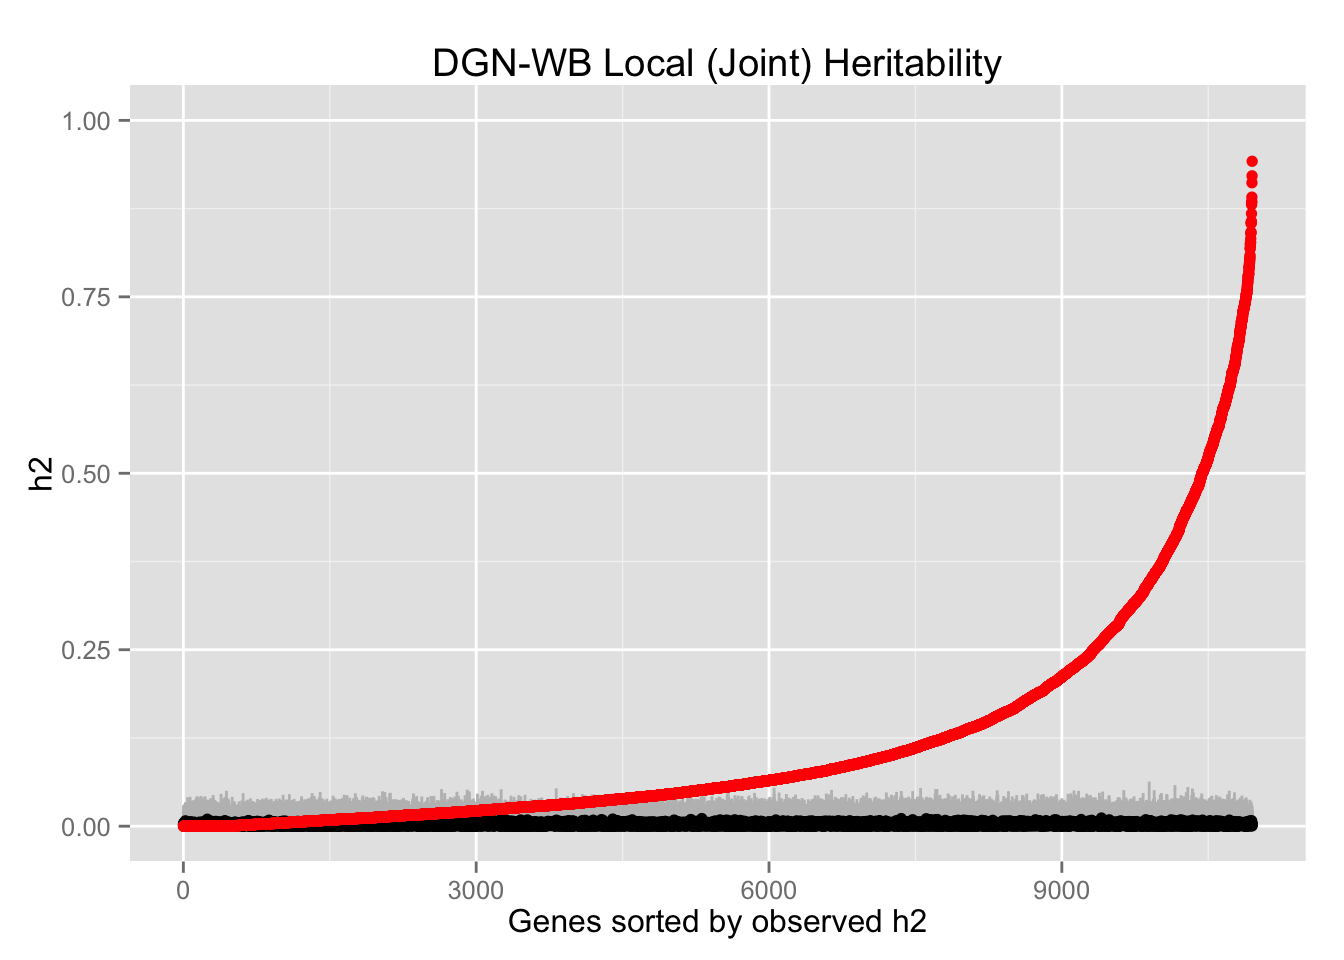
\includegraphics{figs/perms-DGN-localjointh2.png}

\end{frame}

\begin{frame}{100 permutations to determine expected distribution of
h\textsuperscript{2} estimates}

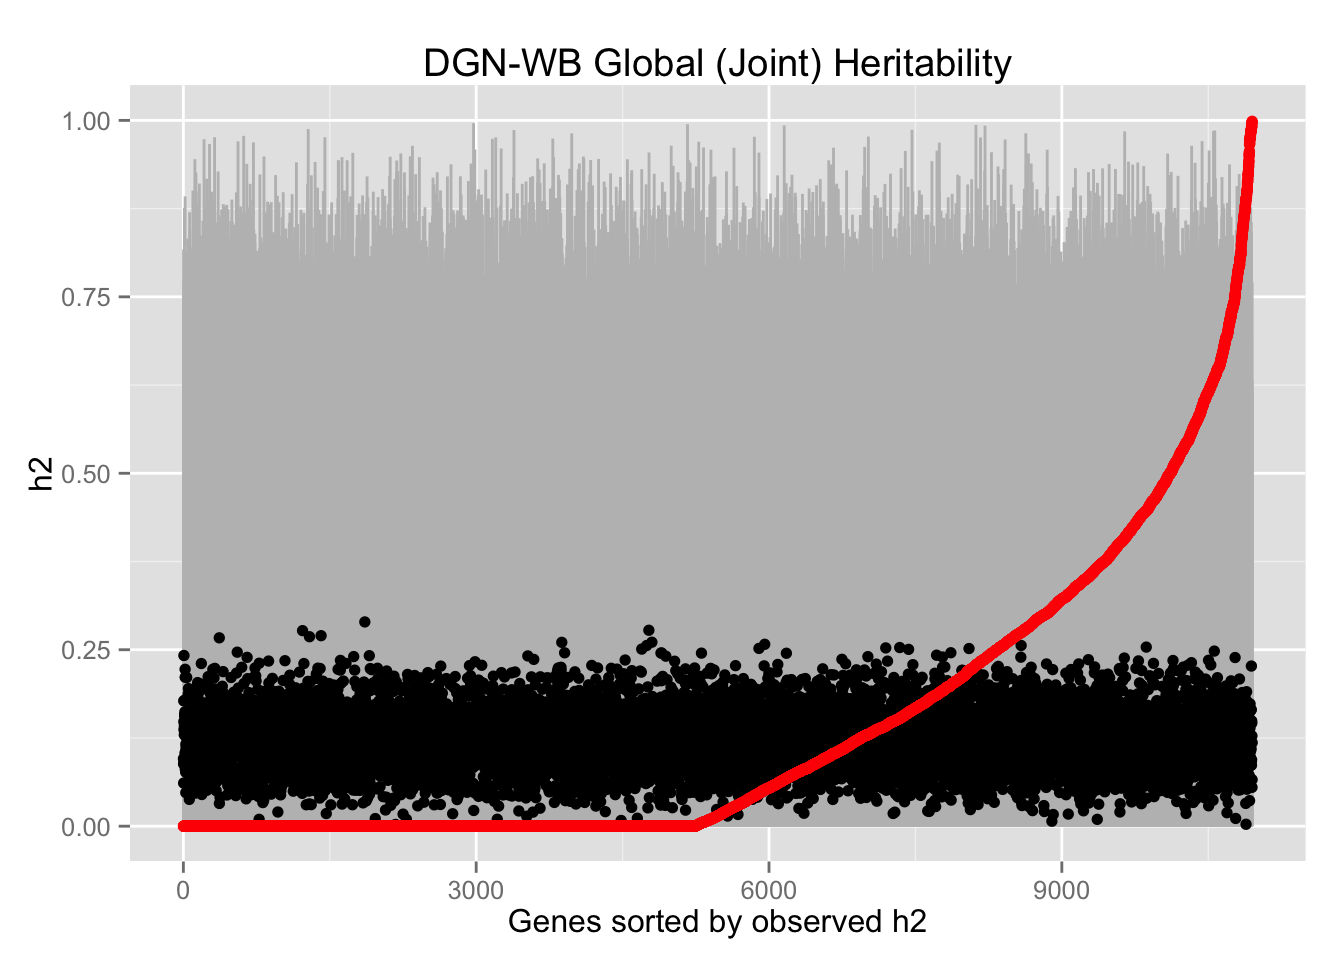
\includegraphics{figs/perms-DGN-globaljointh2.png}

\end{frame}

\begin{frame}{Sort the h\textsuperscript{2} from each permutation}

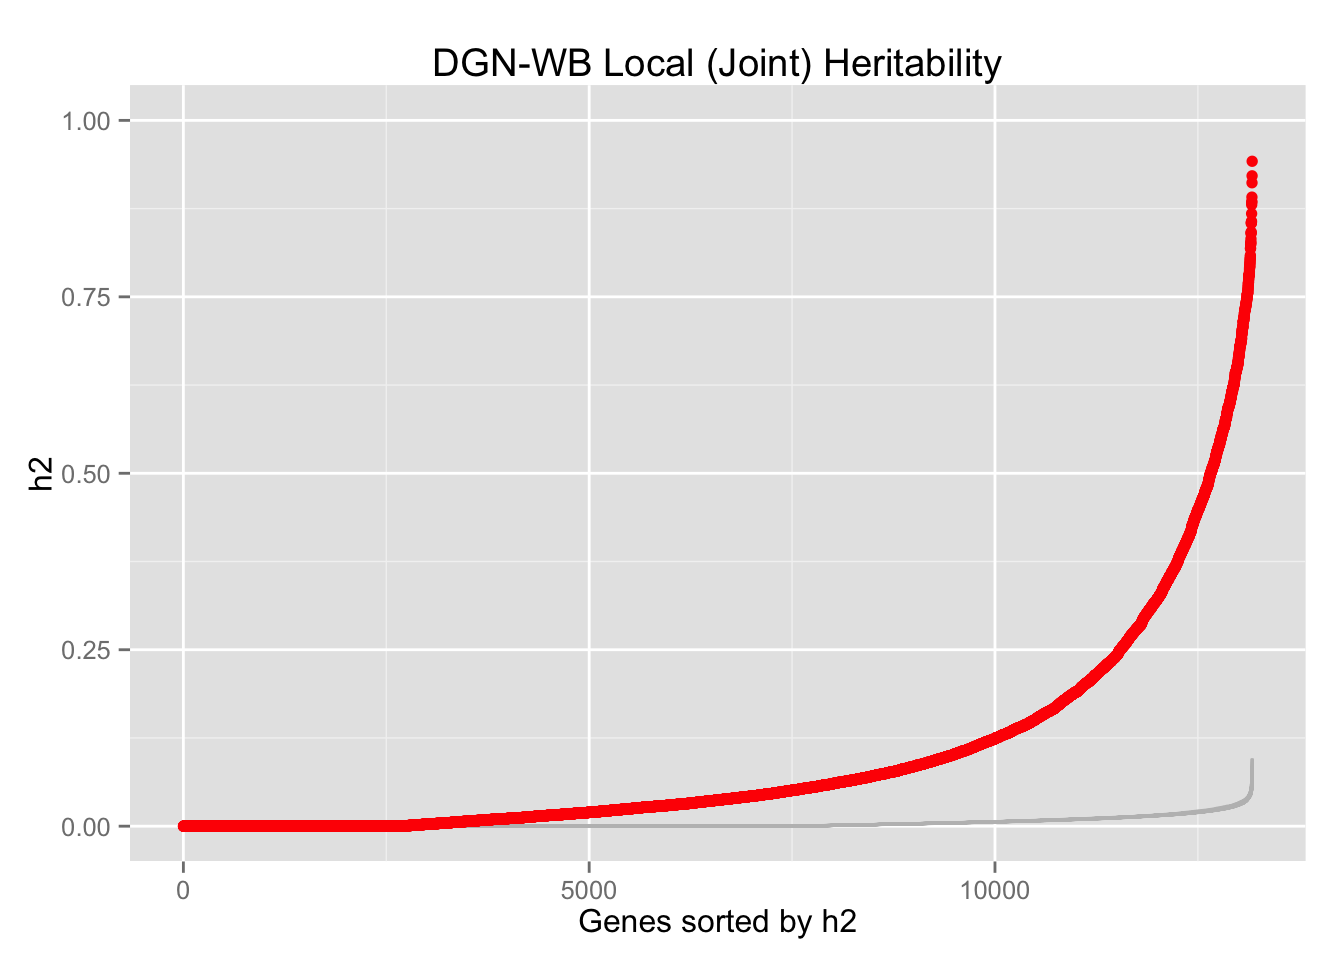
\includegraphics{figs/sortedperms-DGN-localjointh2.png}

\end{frame}

\begin{frame}{Sort the h\textsuperscript{2} from each permutation}

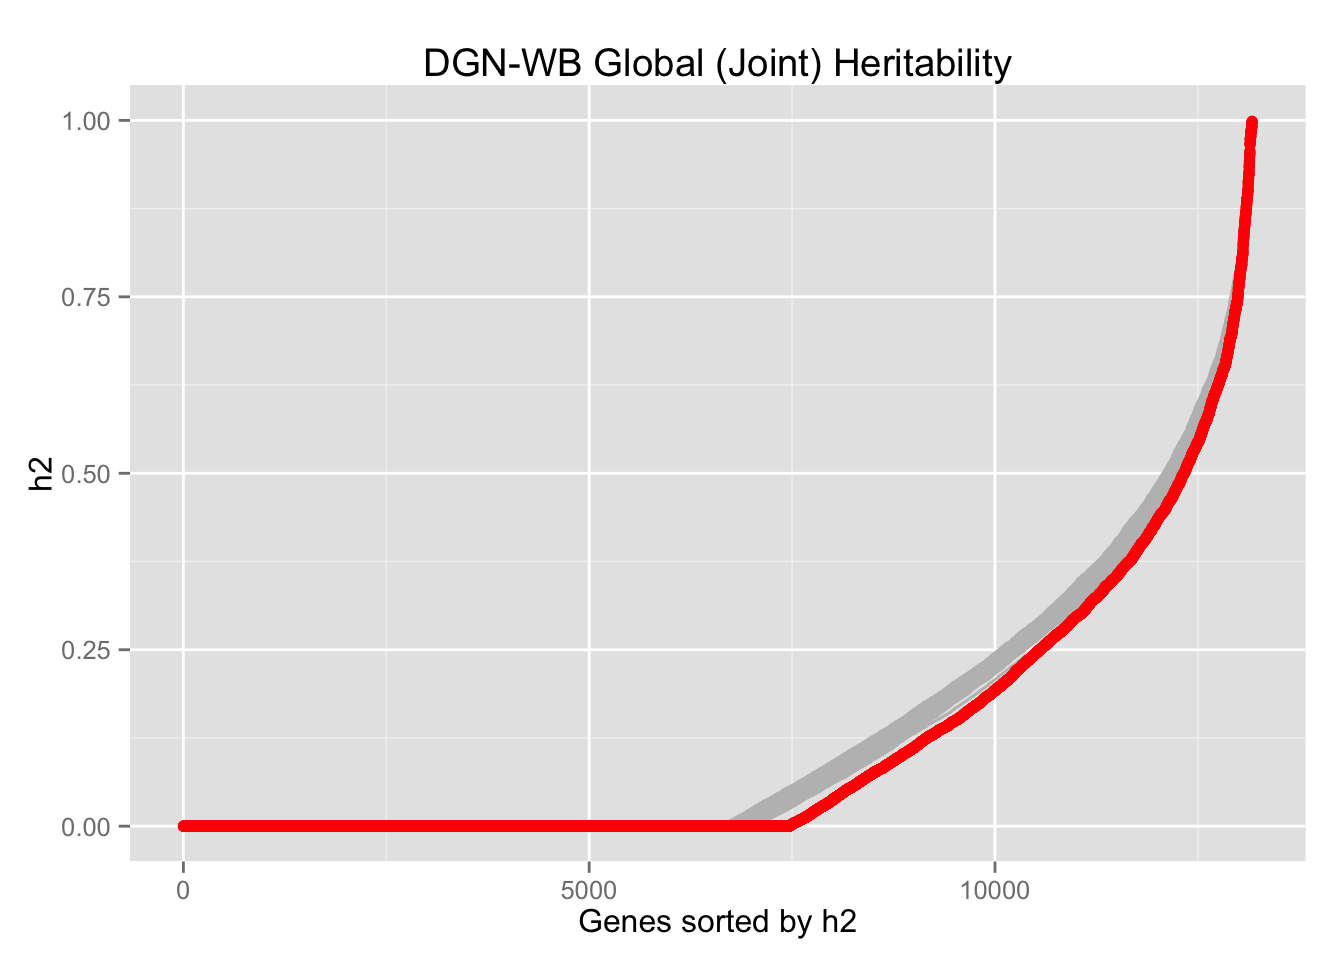
\includegraphics{figs/sortedperms-DGN-globaljointh2.png}

\end{frame}

\begin{frame}{Sort the h\textsuperscript{2} from each permutation}

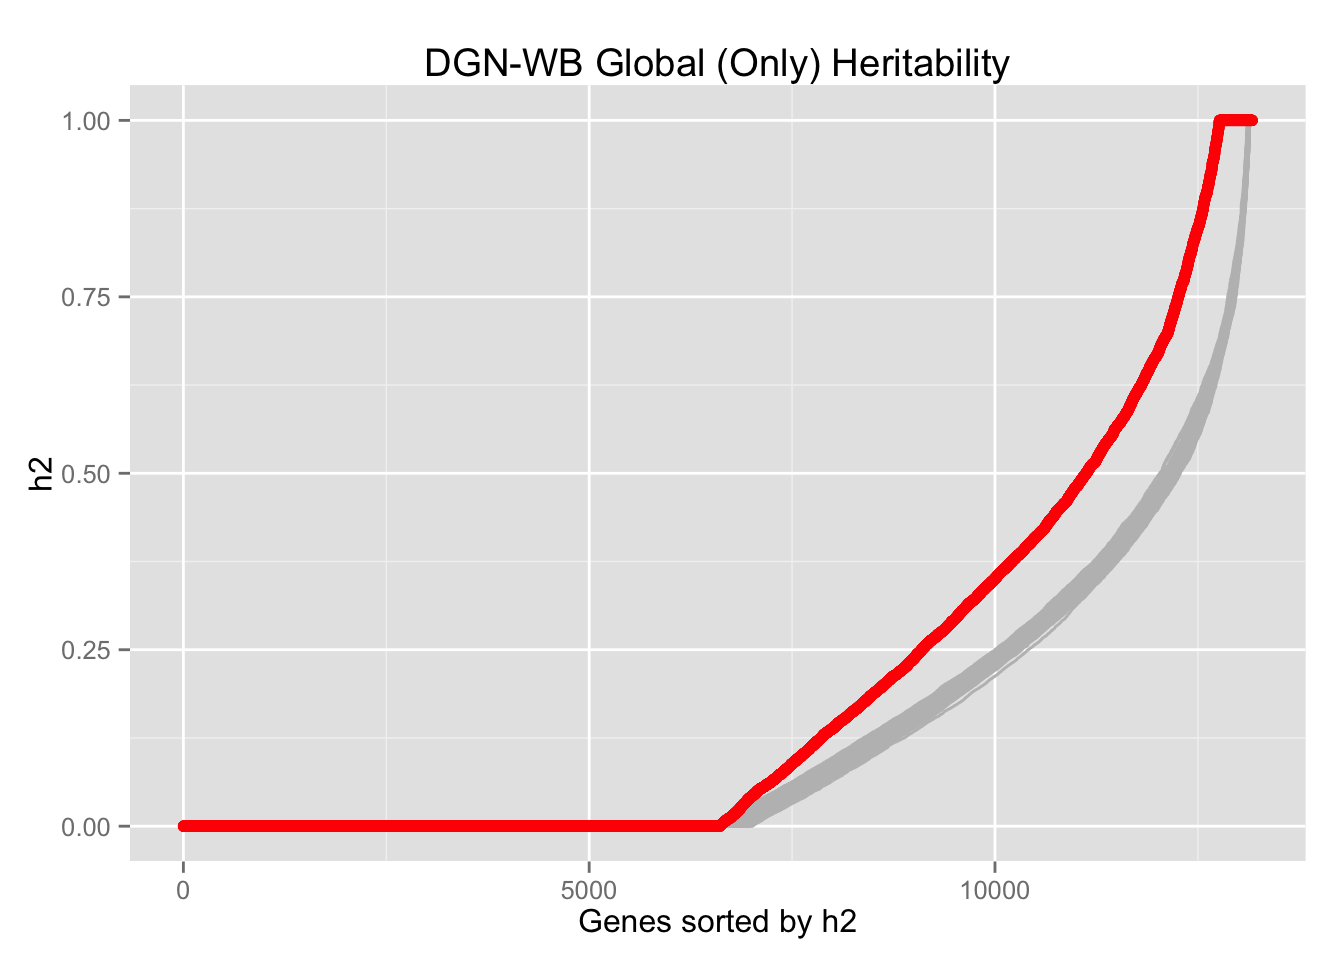
\includegraphics{figs/sortedperms-DGN-globalonlyh2.png}

\end{frame}

\begin{frame}{\emph{cis} vs. \emph{trans} effects}

Try a larger sample to better caputure \emph{trans} effects

\textbf{Framingham Heart Study}

\begin{itemize}
\itemsep1pt\parskip0pt\parsep0pt
\item
  n = 5257
\item
  exon expression array and genotype array
\end{itemize}

\end{frame}

\begin{frame}{sparse vs.~polygenic effects}

\texttt{glmnet} solves the following problem {\[
\min_{\beta_0,\beta} \frac{1}{N} \sum_{i=1}^{N} w_i l(y_i,\beta_0+\beta^T x_i) + \lambda\left[(1-\alpha)||\beta||_2^2/2 + \alpha ||\beta||_1\right],
\]} over a grid of values of {$\lambda$} covering the entire range.

The elastic-net penalty is controlled by {$\alpha$}, and bridges the gap
between lasso ({$\alpha=1$}, the default) and ridge ({$\alpha=0$}). The
tuning parameter {$\lambda$} controls the overall strength of the
penalty.

\small \url{http://web.stanford.edu/~hastie/glmnet/glmnet_alpha.html}

\end{frame}

\begin{frame}{sparse vs.~polygenic effects}

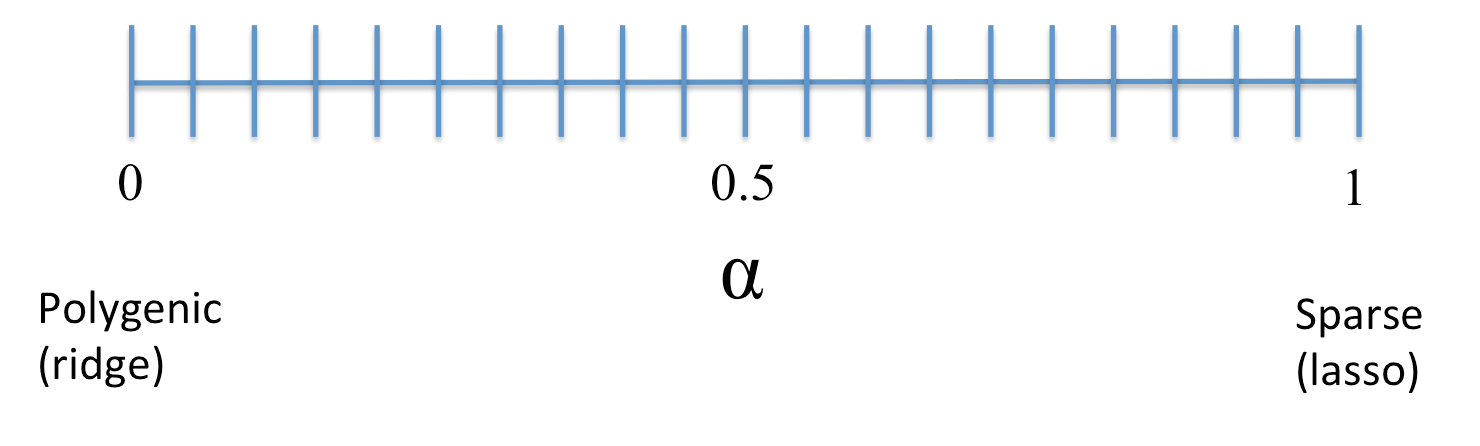
\includegraphics{figs/enline.png}

For each gene, determine {$\alpha$} with best 10-fold CV predictive
performance using \emph{cis} SNPs.

\end{frame}

\begin{frame}{Predictive performance consistent across most alphas}

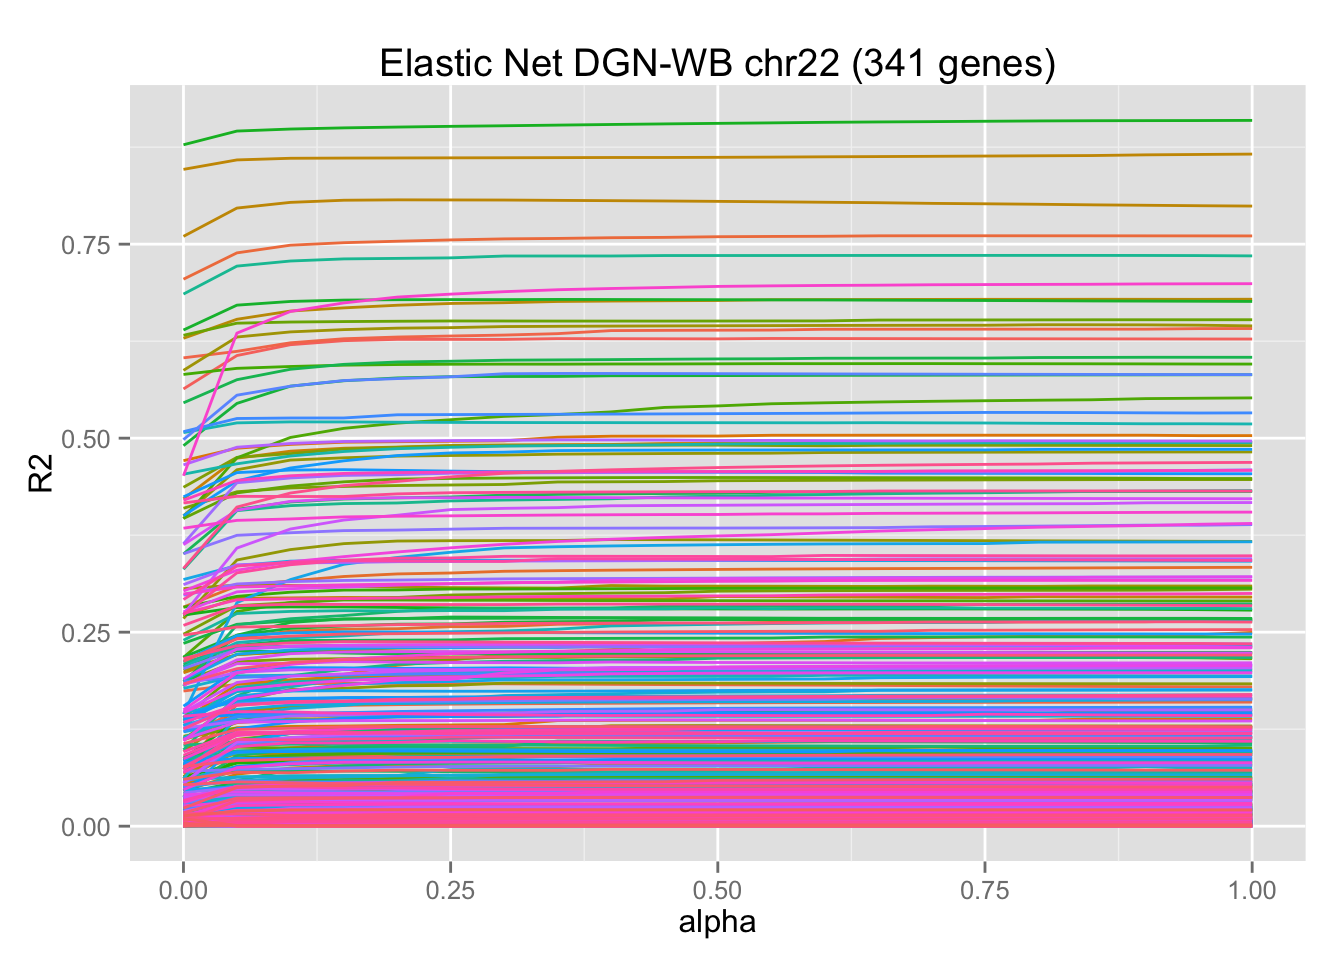
\includegraphics{figs/chr22EN.png}

\end{frame}

\begin{frame}{Predictive performance consistent between {$\alpha$}=0.5
and {$\alpha$}=1}

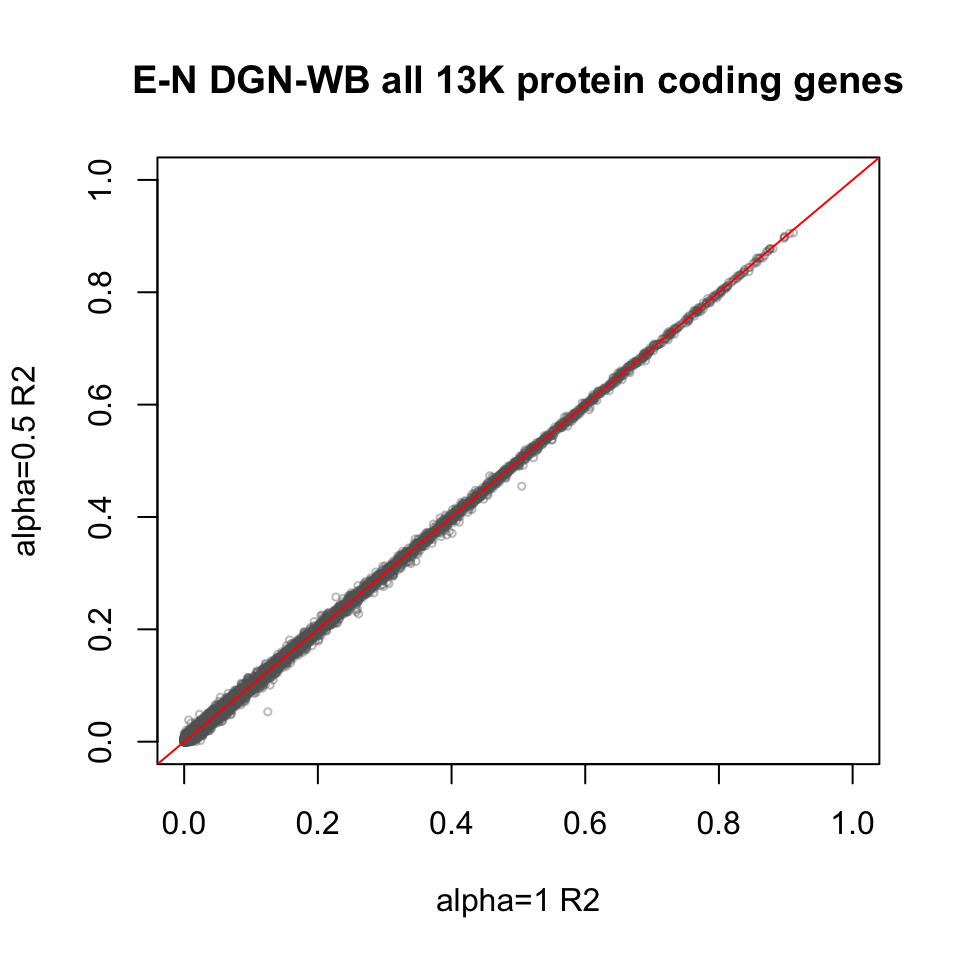
\includegraphics{figs/DGN-EN-alpha-05v10.png}

\end{frame}

\begin{frame}{Also tested Polyscore predictive performance using 10-fold
CV}

$expression = \sum\hat{w}*gt$

Single variant linear regression coefficients ($w$) at several P-value
thresholds included in the additive model:

\begin{itemize}
\itemsep1pt\parskip0pt\parsep0pt
\item
  $P<0.0001$
\item
  $P<0.001$
\item
  $P<0.01$
\item
  $P<0.05$
\item
  $P<0.5$
\item
  $P<1$
\end{itemize}

\end{frame}

\begin{frame}{Polyscore (\emph{cis} SNPs only) predictive performance}

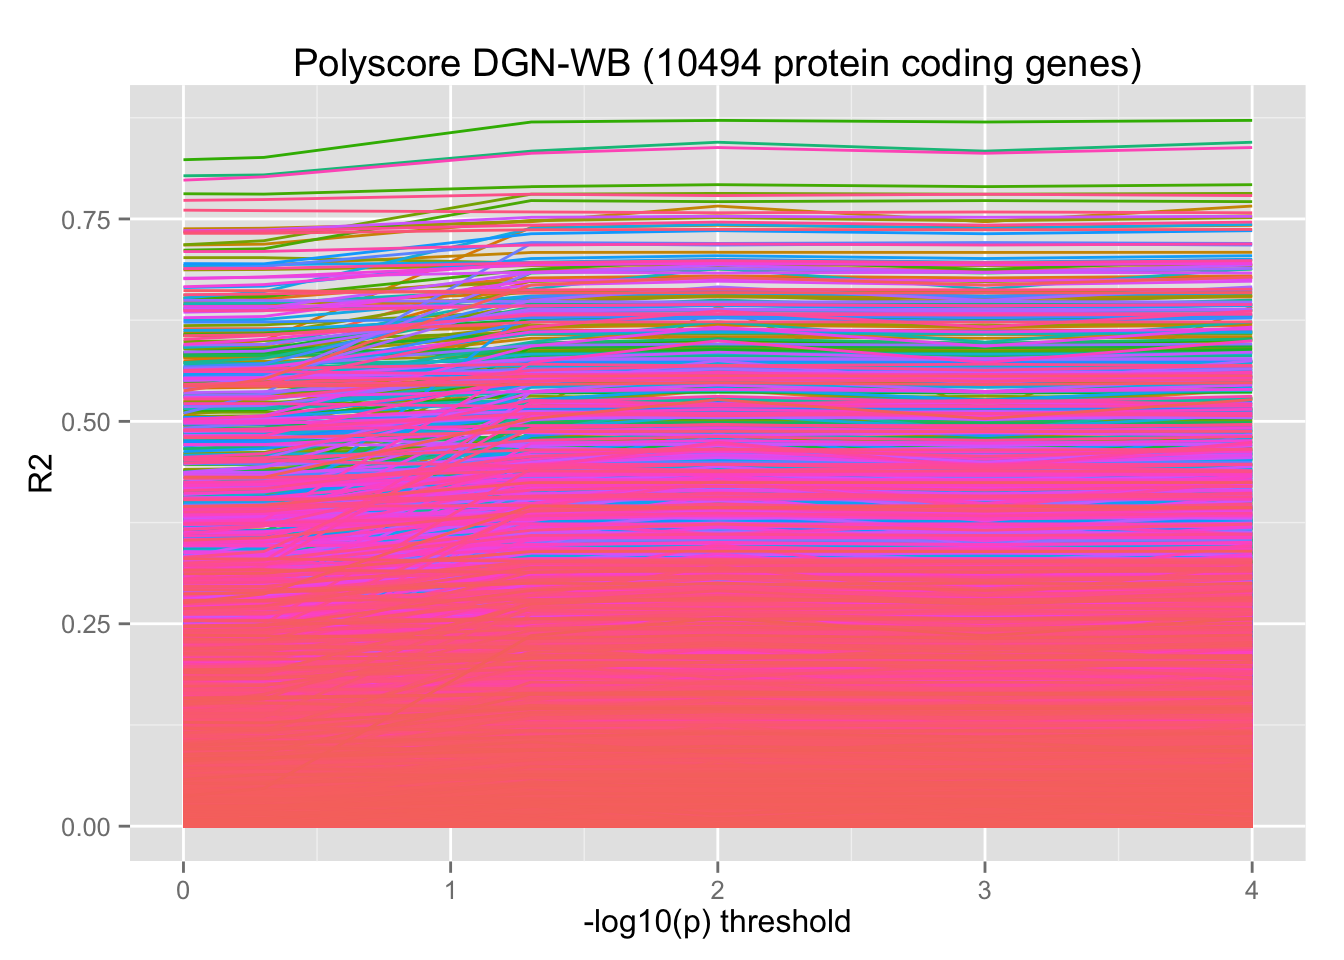
\includegraphics{figs/psDGN.png}

\end{frame}

\begin{frame}{Polyscore (\emph{cis} SNPs only) predictive performance}

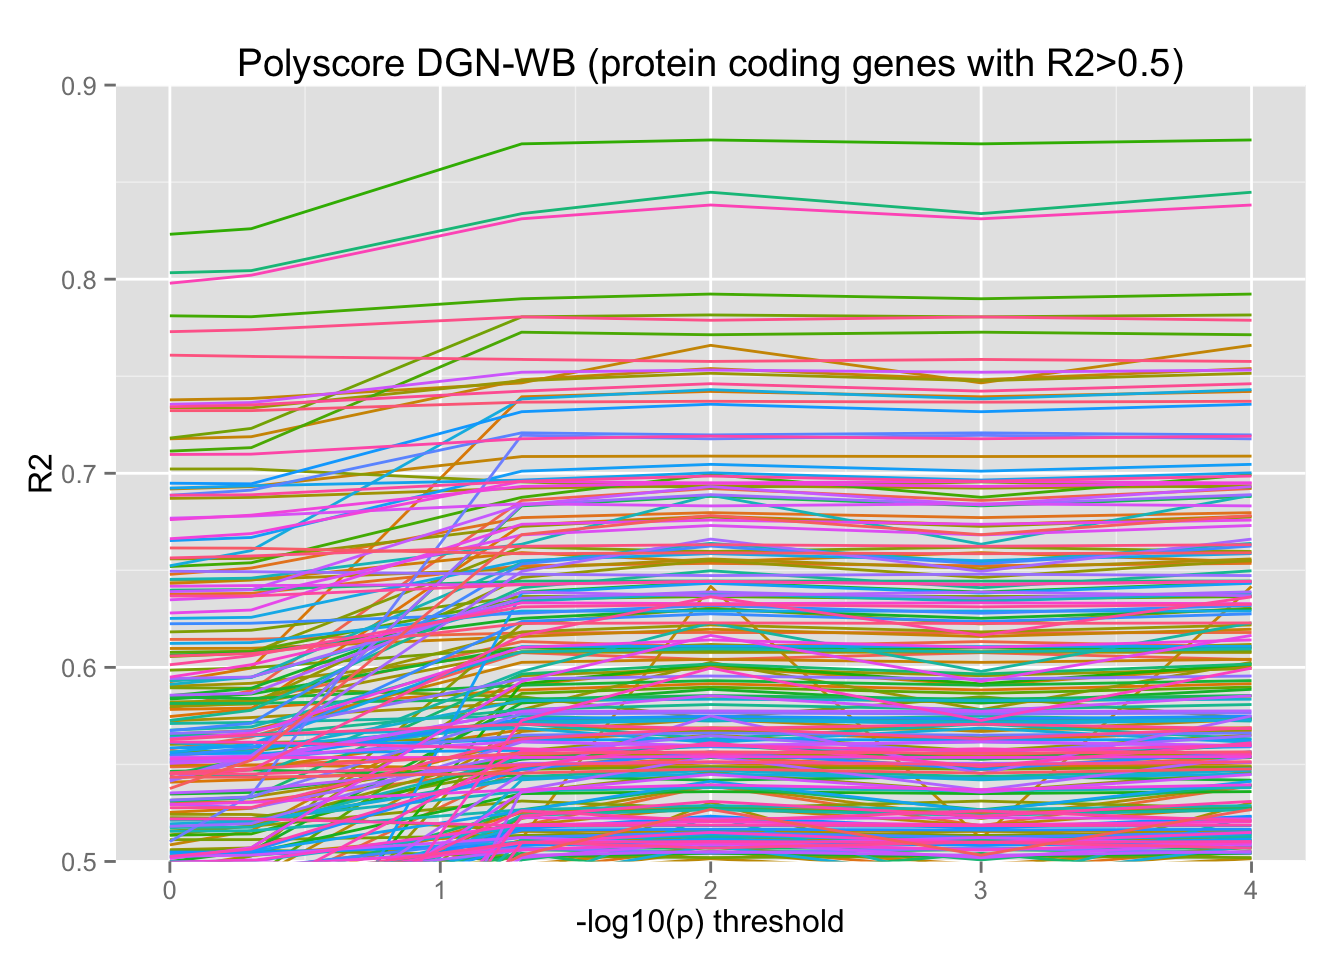
\includegraphics{figs/psDGN-R205.png}

\end{frame}

\begin{frame}{LASSO predicts gene expression better than Polyscore}

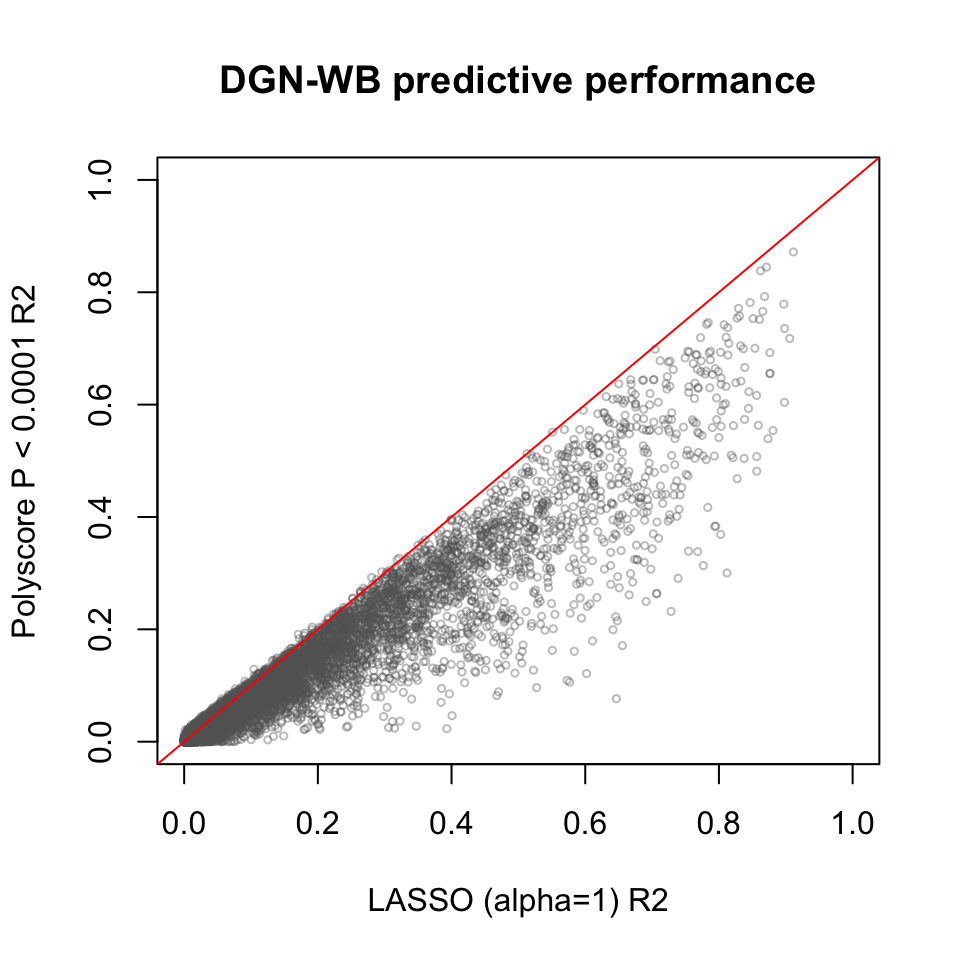
\includegraphics{figs/PSvLASSO.png}

\end{frame}

\begin{frame}{For robustness, consider EN (alpha=0.5) for PrediXcan}

\begin{columns}[c]  %the "c" option specifies center vertical alignment
\column{.5\textwidth}  %column designated by a command
  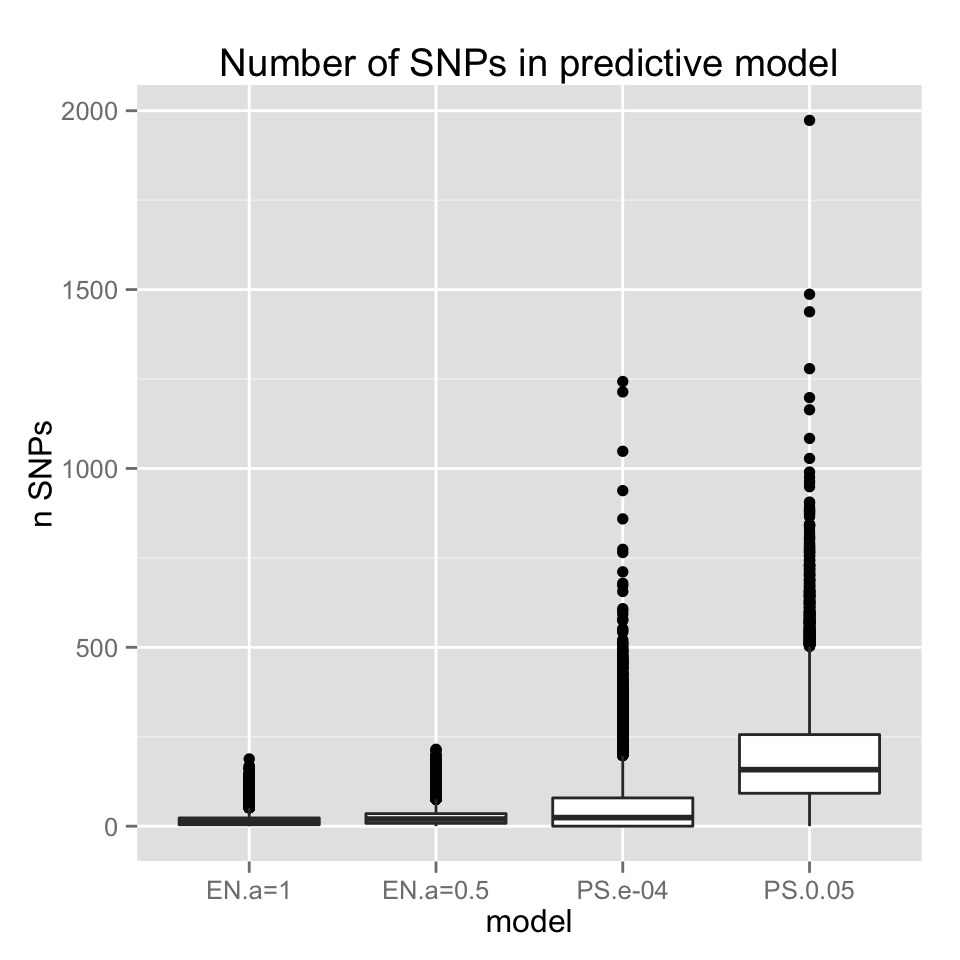
\includegraphics[height=3in]{figs/nsnps.png}
\column{.5\textwidth}
  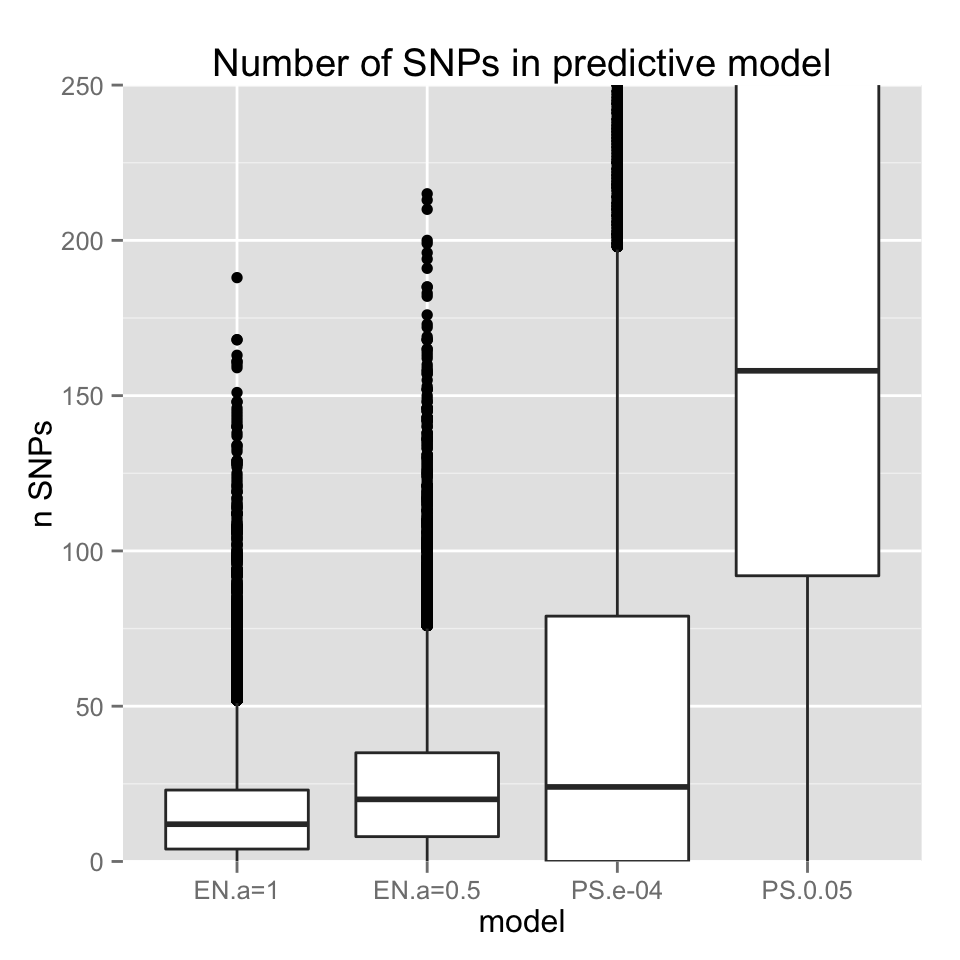
\includegraphics[height=3in]{figs/nsnpsZoom.png}
\end{columns}

\end{frame}

\begin{frame}{LASSO predictive performance reaches (or exceeds?) local
h\textsuperscript{2} of most genes}

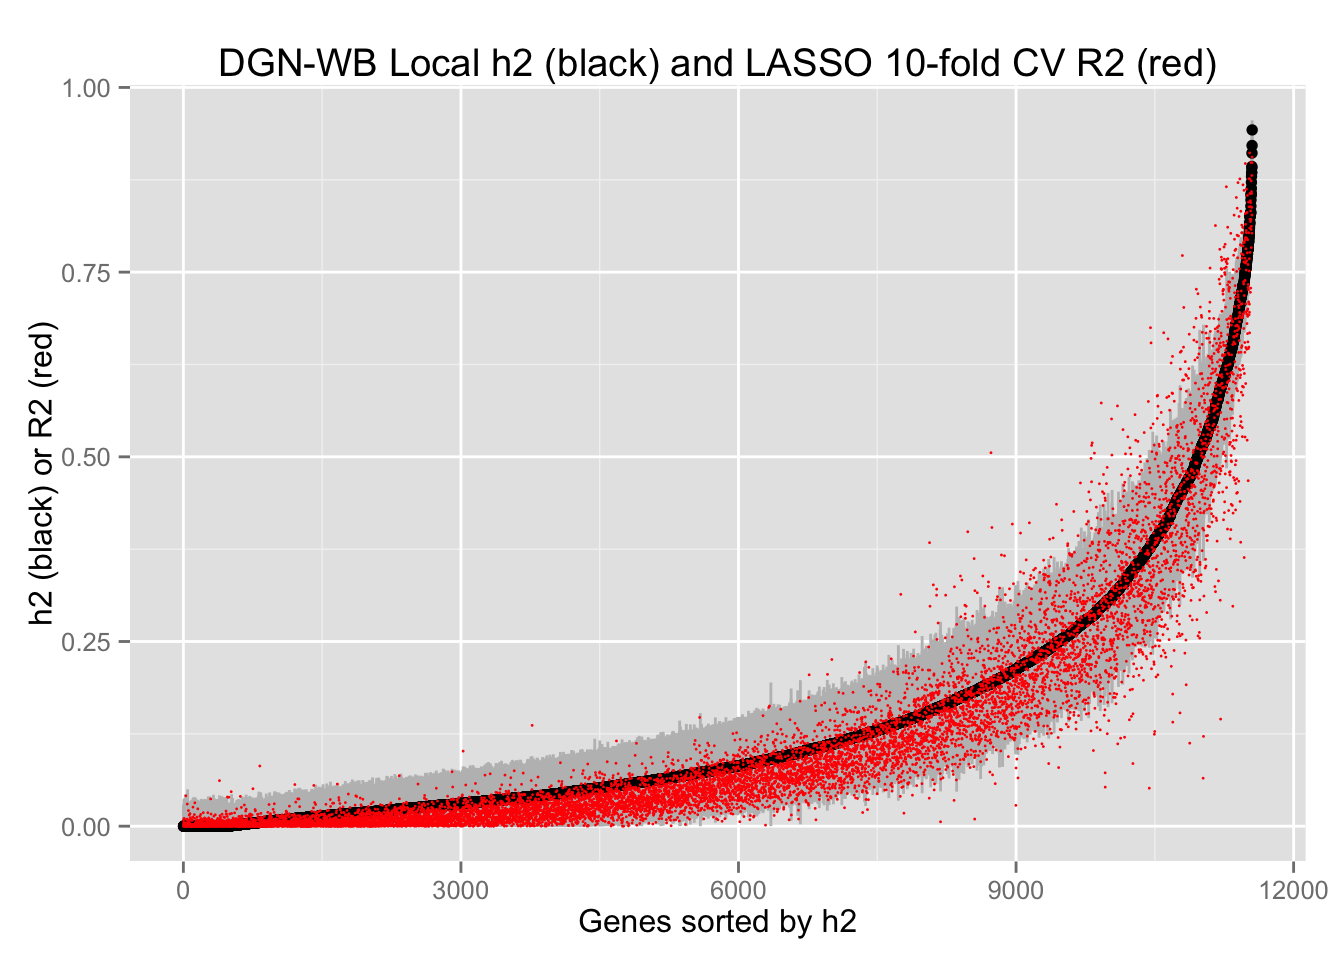
\includegraphics{figs/DGN-h2-lassoR2.png}

\end{frame}

\begin{frame}{Polyscore predictive performance does not reach local
h\textsuperscript{2} of many genes}

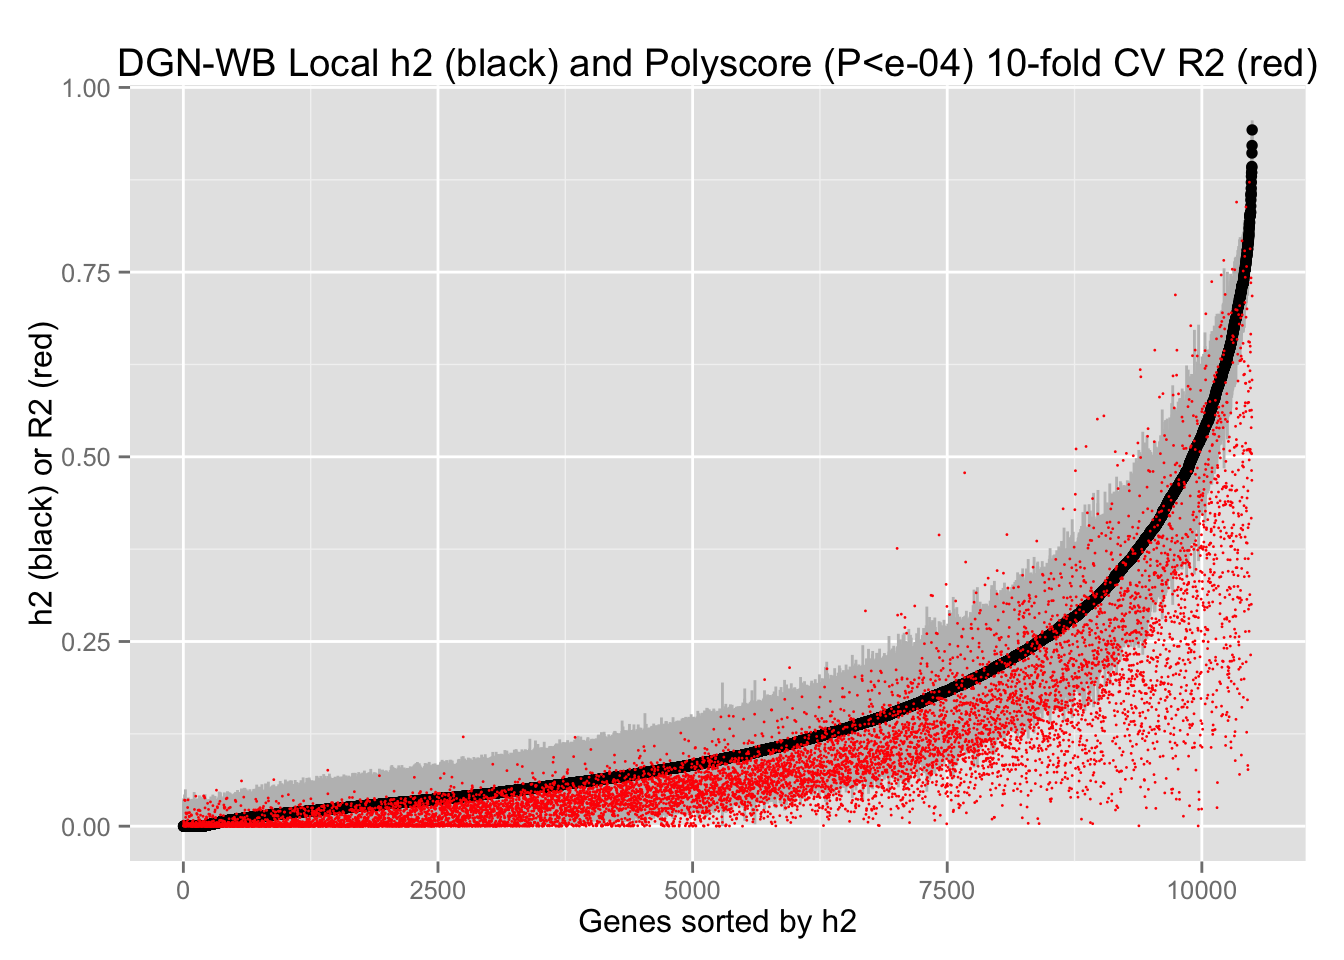
\includegraphics{figs/DGN-h2-polyscoreR2.png}

\end{frame}

\begin{frame}{cross-tissue vs.~tissue-specific effects with GTEx}

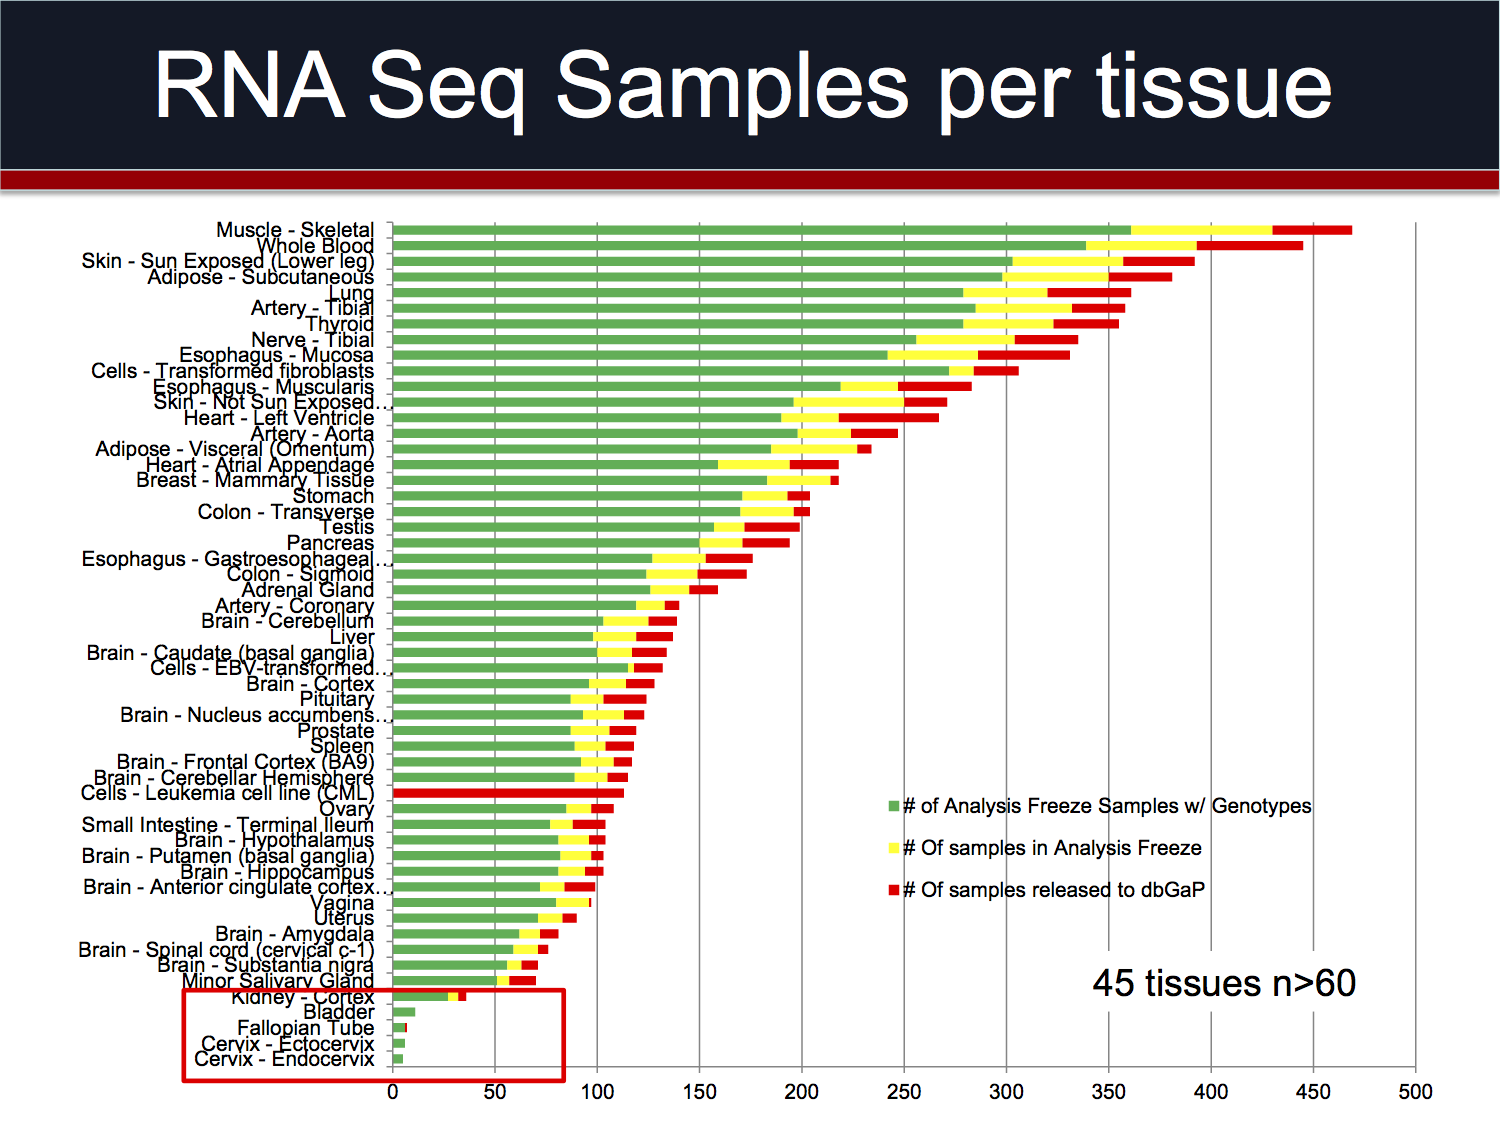
\includegraphics{figs/gtex.png}

\end{frame}

\begin{frame}[fragile]{Modeling cross-tissue expression}

Linear mixed effect model using \texttt{GTEx\_Data\_2014-06-13} release

\begin{itemize}
\itemsep1pt\parskip0pt\parsep0pt
\item
  8555 tissues across 544 subjects
\item
  limited to \textasciitilde{}17K protein coding genes
\end{itemize}

\begin{Shaded}
\begin{Highlighting}[]
\KeywordTok{library}\NormalTok{(lme4)}

\NormalTok{fit <-}\StringTok{ }\KeywordTok{lmer}\NormalTok{(expression ~}\StringTok{ }\NormalTok{(}\DecValTok{1}\NormalTok{|SUBJID) +}\StringTok{ }\NormalTok{TISSUE }
\NormalTok{+}\StringTok{ }\NormalTok{GENDER +}\StringTok{ }\NormalTok{PEERs) }

\CommentTok{#cross-tissue expression}
\NormalTok{fitranef <-}\StringTok{ }\KeywordTok{ranef}\NormalTok{(fit) }

\CommentTok{#tissue-specific expression}
\NormalTok{fitresid <-}\StringTok{ }\KeywordTok{resid}\NormalTok{(fit) }
\end{Highlighting}
\end{Shaded}

\end{frame}

\begin{frame}{Estimating heritability with GCTA}

Tested two genetic relationship matrix (GRM) models for each expressed
gene

\begin{itemize}
\itemsep1pt\parskip0pt\parsep0pt
\item
  localGRM (SNPs within 1 Mb of gene)
\item
  localGRM + globalGRM (all SNPs)
\end{itemize}

First pass: estimated h\textsuperscript{2} of cross-tissue expression
and tissue-specific expression in the 7 tissues with the most samples

\end{frame}

\begin{frame}{GCTA heritability: localGRM h\textsuperscript{2}}

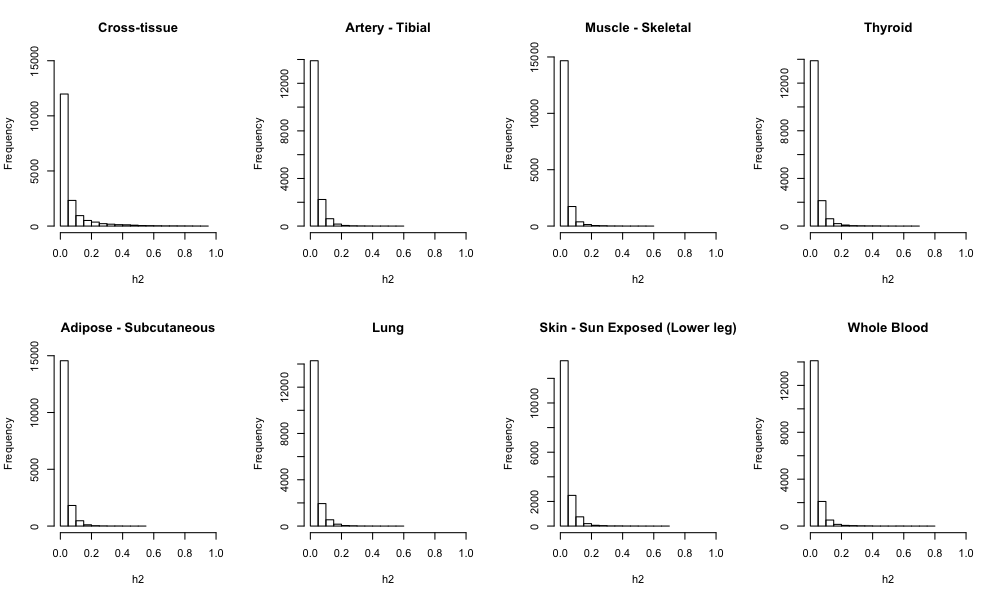
\includegraphics{figs/hist_GTEx_localGRM_h2_2015-02-18.png}

\end{frame}

\begin{frame}{GCTA heritability: localGRM h\textsuperscript{2}
\textbf{ZOOM}}

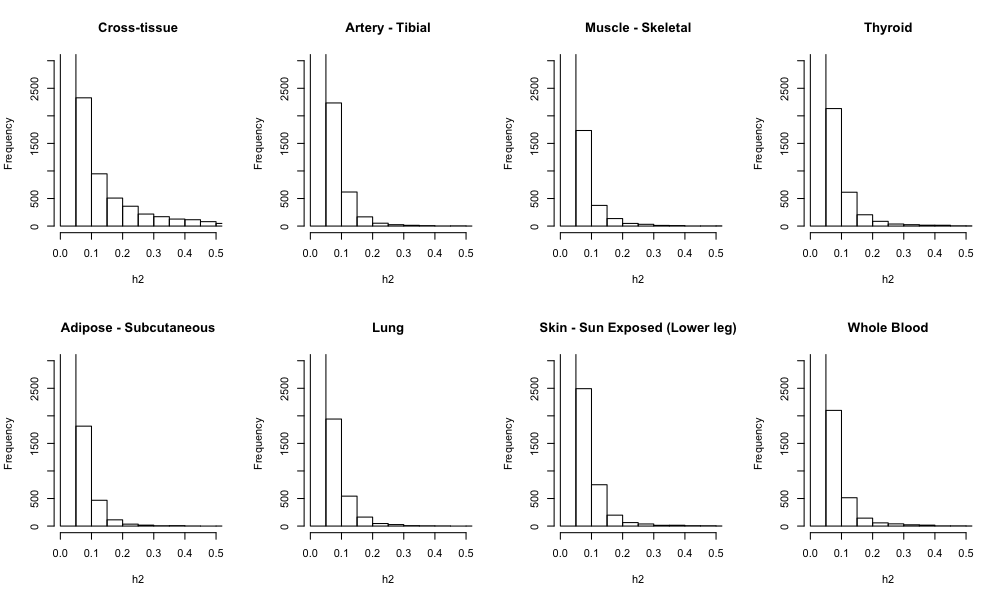
\includegraphics{figs/hist_GTEx_localGRM_h2_ylim3000_2015-02-18.png}

\end{frame}

\begin{frame}{GCTA heritability: localGRM p-values}

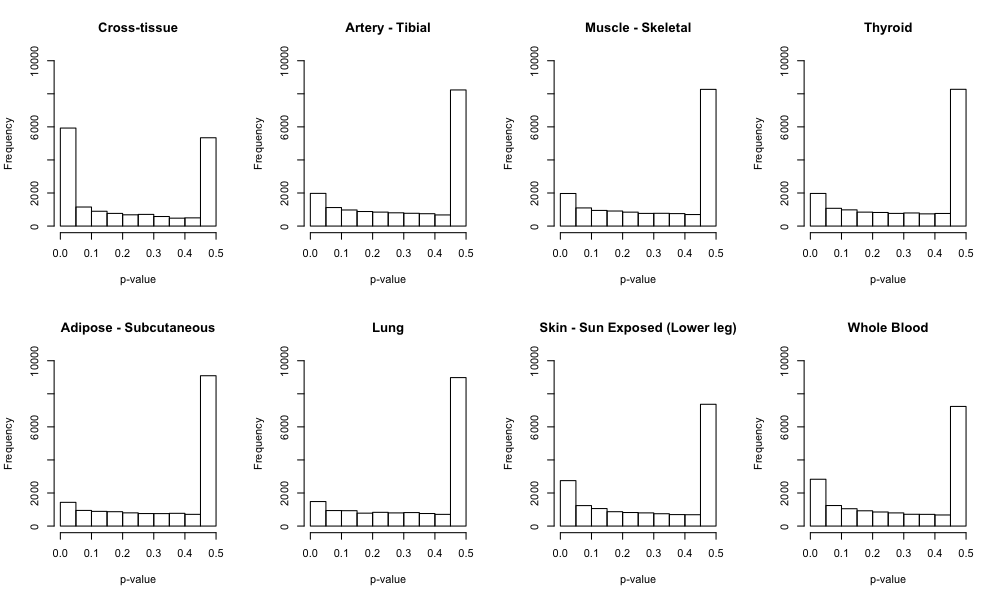
\includegraphics{figs/hist_GTEx_localGRM_p_2015-02-18.png}

\end{frame}

\begin{frame}{GCTA joint heritability: localGRM + globalGRM
h\textsuperscript{2}}

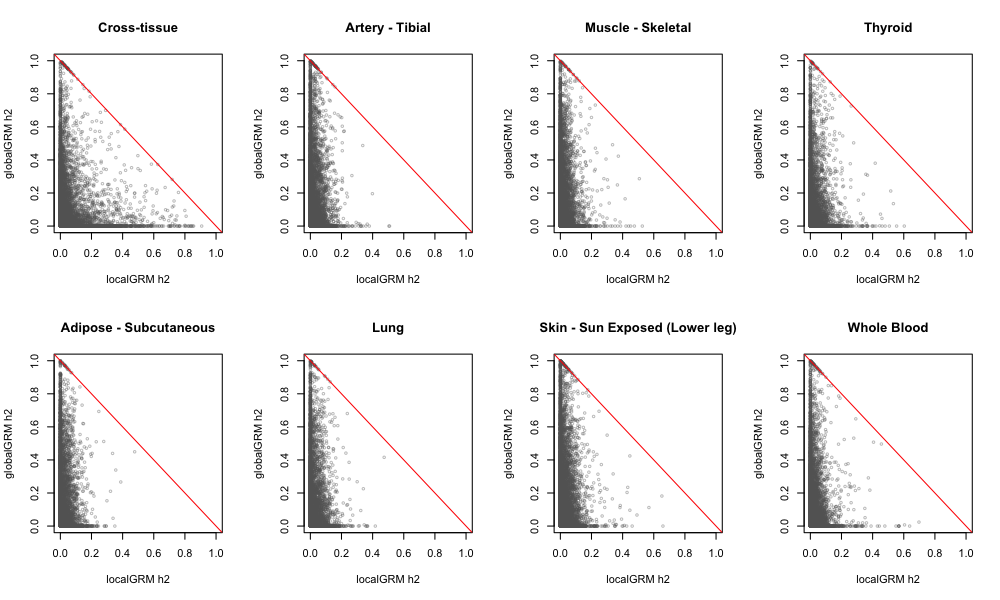
\includegraphics{figs/scatter_GTEx_localGRM_globalGRM_h2_2015-02-18.png}

\end{frame}

\begin{frame}{GCTA joint heritability: localGRM + globalGRM
h\textsuperscript{2}}

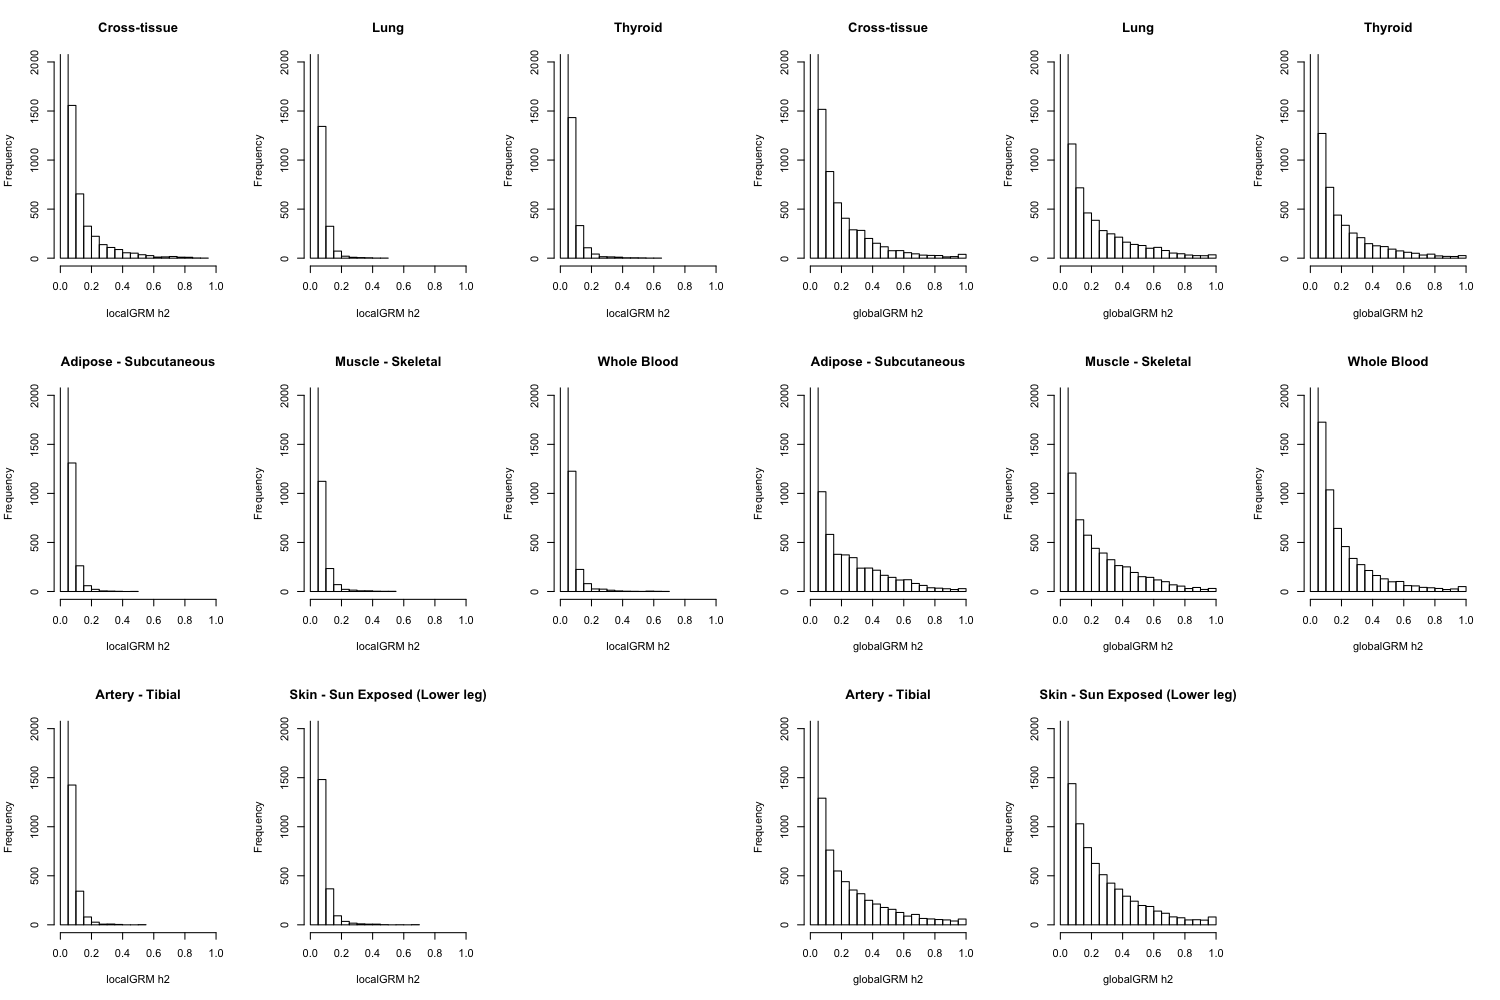
\includegraphics{figs/hist_GTEx_localGRM_globalGRM_h2_2015-02-18.png}

\end{frame}

\begin{frame}{GCTA joint heritability: localGRM + globalGRM SE}

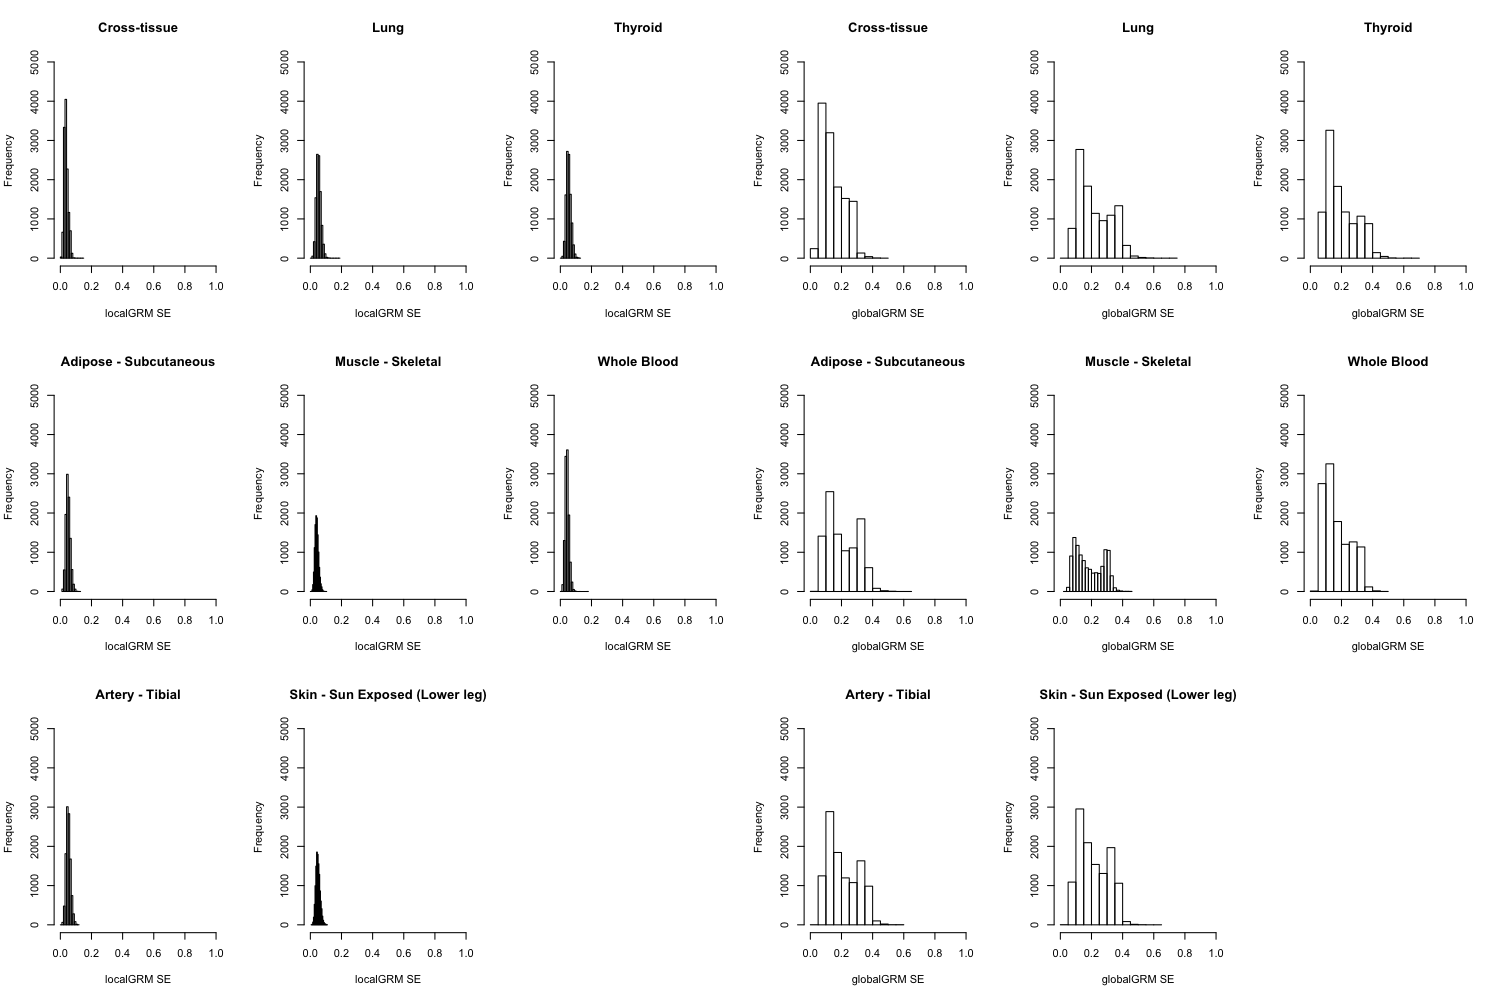
\includegraphics{figs/hist_GTEx_localGRM_globalGRM_se_2015-02-18.png}

\end{frame}

\begin{frame}{Summary}

\textbf{\emph{cis} vs. \emph{trans} effects}

\begin{itemize}
\itemsep1pt\parskip0pt\parsep0pt
\item
  \emph{cis} effects are easily detected: 37\% of DGN-WB genes have
  local h\textsuperscript{2} \textgreater{} 0.1, 81\% have local
  h\textsuperscript{2} \textgreater{} 0.01
\item
  good estimates of \emph{trans} h\textsuperscript{2} will require
  larger n
\end{itemize}

\textbf{sparse vs.~polygenic effects}

\begin{itemize}
\itemsep1pt\parskip0pt\parsep0pt
\item
  \emph{cis} effects are mostly sparse (LASSO beats ridge and polyscore)
\end{itemize}

\textbf{cross-tissue vs.~tissue-specific effects}

\begin{itemize}
\itemsep1pt\parskip0pt\parsep0pt
\item
  GTEx cross-tissue local h\textsuperscript{2} is greater than
  tissue-specific local h\textsuperscript{2}
\end{itemize}

\end{frame}

\end{document}
